% !TeX root = handout.tex

% !TeX root = ../notes.tex

\documentclass[
    a4paper,
    12pt,
]{article}

% !TeX root = ../handout.tex

\usepackage[english,ngerman]{babel}
\usepackage[utf8]{inputenc}

\usepackage[htt]{hyphenat}

\usepackage{soul}


\usepackage[figurename=Fig.]{caption}
\makeatletter
\renewcommand{\fnum@figure}{Abb. \thefigure}
\makeatother
\addto\captionsngerman{\renewcommand{\figurename}{Abb.}}

% !TeX root = ../presentation.tex

\title{Data Spaces am Beispiel von Solid}

% \subtitle[SUBTITLE]
%     {FORMATTED\\SUBTITLE}

\date{07. Juli 2025}
\author[N. Schramm]{Nico Schramm}

\titlegraphic{\flushright
\includegraphics[width=2cm]{./assets/htwk_logo.png}}

\newcommand{\module}{Innovative Methoden für Software Engineering der Zukunft}
\newcommand{\prof}{Prof. Dr. Andreas Both}

\newcommand{\faculty}{Fakultät Informatik und Medien}
\newcommand{\university}{Hochschule für Technik, Wirtschaft und Kultur Leipzig}

\institute{\module\\
  \prof\\~\\
  \faculty\\
  \university}

\newcommand{\repourl}{https://github.com/nicosrm/25-sez-solid}

\hypersetup{
  % PDF metadata
  pdfauthor={Nico Schramm},
  pdftitle={Data Spaces am Beispiel von Solid},
  pdfsubject={Präsentation},
  % hyperref colouring
  colorlinks,
  allcolors=.,
  urlcolor=blue,
  citecolor=cyan
}


\makeatletter
\hypersetup{
    pdfauthor={\@author},
    pdftitle={\@title},
    pdfsubject={\subject},
    citecolor=blue
}
\makeatother


\begin{document}

\maketitle

\begin{abstract}
  % !TeX root = ../handout.tex

\blindtext

\end{abstract}

% content
% !TeX root = ../handout.tex

\section{Einleitung und Motivation}

\begin{itemize}
    \item aktueller Stand
    \begin{itemize}
        \item zentralisiert
        \item Datensilos, Datenmissbrauch, veraltete Daten
    \end{itemize}
    
    \item industrieller Kontext
    \begin{itemize}
        \item Daten als strategische Ressource
        \item Supply Chain (Act) Bedenken beim Teilen von Daten
    \end{itemize}

    \item Vision
    \begin{itemize}
        \item ad"=hoc"=Zusammenschaltung von Geschäftsprozessen, Daten"= / Anwendungsintegration
        \item Aktualität und Konsistenz von Daten
        \item Kostenreduktion, Wirtschaftlichkeit
        \item Vertrauen
    \end{itemize}
\end{itemize}

\cite{sambraSolidPlatformDecentralized2016,bothSolidBasedB2BData2025,mecklerWebLinkedData2023,mollerIndustrialDataEcosystems2024}

% (kurze Zusammenfassung der Struktur der Belegarbeit)
% Diese Arbeit ist folgendermaßen strukturiert. 
% In Kapitel ... 
% ...
% ...
% Abschließend ...

% !TeX root = ../handout.tex

\section{Grundlagen}
% Begriffe und Definitionen

\begin{itemize}
    \item zentralisiertes Daten"=Konzept
    \item Datensouveränität
    \item RDF, Semantic Web, Linked Data
\end{itemize}

% !TeX root = ../presentation.tex

\section{Data Spaces}

\begin{frame}{Inter-Organisational Information Systems (IOIS) \footnotesize\cite{mollerIndustrialDataEcosystems2024}}
    \begin{columns}
        \begin{column}{0.6\textwidth}
            \begin{itemize}
                \item \alert{bilaterale} Beziehungen, bspw. Lieferketten
                \item tiefe Integration, automatisiertes Data Sharing
                \item zweckgebunden, bspw. Koordinierung und Optimierung von Lieferketten
                % \item Mittel zum Zweck
                
                \item<2-> mangelndes Vertrauen, streng formalisierte Nutzungsrichtlinien
                \item<2-> keine Daten teilen? $\to$ Ineffizienz $\to$ Verlust
                \item<2-> Herausforderungen bei Skalierung % Datenaustausch, Kontrolle
            \end{itemize}
        \end{column}
        
        \begin{column}{0.4\textwidth}
            \begin{figure}
                
\includegraphics[height=0.5\textheight]{./assets/iois_architecture.drawio.pdf}
                \caption{IOIS Architektur}
            \end{figure}
        \end{column}
    \end{columns}
\end{frame}


\begin{frame}{Data Intermediaries \footnotesize\cite{mollerIndustrialDataEcosystems2024}}
    \begin{columns}
        \begin{column}{0.6\textwidth}
            \begin{itemize}
                % \item dynamisch, geteilter Zweck
                \item Gleichgewicht zwischen erhaltenem und gegebenem Aufwand
                \item Daten als strategische Ressource % statt Mittel zum Zweck
                % \item ermöglichen neue Geschäfte und Optimierung von Prozessen
                
                \item<2-> Interaktion und Kooperation \alert{multilateraler} Akteure
                \item<2-> Data User, Data Provider, Data Intermediary
                
                \item<3-> offener, dynamischer Datenaustausch
                \item<3-> Netzwerkeffekte, Förderung von Innovation
            \end{itemize}
        \end{column}
        
        \begin{column}{0.4\textwidth}
            \begin{figure}
                \centering
                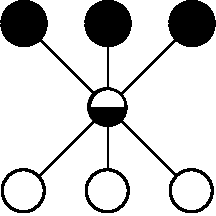
\includegraphics[height=0.5\textheight]{./assets/industrial_de_architecture.drawio.pdf}
                \caption{Industrial Data Ecosystems mit Data Intermediary}
            \end{figure}
        \end{column}
    \end{columns}
\end{frame}


\begin{frame}{Data Spaces \footnotesize\cite{mollerIndustrialDataEcosystems2024}}
    \begin{columns}
        \begin{column}{0.6\textwidth}
            \begin{itemize}
                \item Vereinen von IOIS und Data Intermediaries
                \item dezentrale Speicherung von Daten bei Provider
                
                % TODO: ???
                \item<2-> \emph{Data Space Connectors} für bilateralen Datenaustausch % vgl. IOIS
                \item<2-> Zusammenbringen von Data User und Provider % vgl. Data Intermediary
                
                \item<3-> technische Garantie von Datensouveränität
                % -> Überwindung betriebl. Barrieren
                % Kontrolle über Zugriff und Verwendung bei Provider
                \item<3-> geteilter Raum für vertrauenswürdiges Data Sharing $\to$ Optimierung, Innovation
            \end{itemize}
        \end{column}
        
        \begin{column}{0.4\textwidth}
            \begin{figure}
                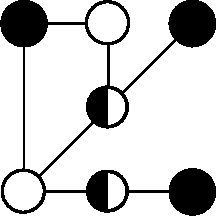
\includegraphics[height=0.5\textheight]{./assets/data_space_architecture.drawio.pdf}
                \caption{Data Space Architektur}
            \end{figure}
        \end{column}
    \end{columns}
\end{frame}


\begin{frame}[c]{Data Spaces II \footnotesize\cite{mollerIndustrialDataEcosystems2024}}
    % verteilt by Design --> Daten bleiben bei Quelle, d.h. Data Provider
    % Zugang nur gewährt, wenn notwendig
    \vspace{1.5em}
    \begin{figure}
        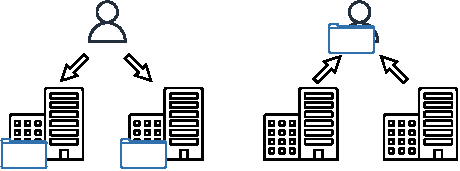
\includegraphics[height=0.6\textheight]{./assets/central_vs_decentral.drawio.pdf}
        \caption{Symbolbild: zentralisierte vs. dezentralisierte Datenspeicherung}
    \end{figure}
\end{frame}


\begin{frame}{Data Spaces III \footnotesize\cite{mollerIndustrialDataEcosystems2024}}
    \begin{columns}
        \begin{column}{0.6\textwidth}
            \begin{itemize}
                \item dezentralisierte Datenspeicherung
                \begin{itemize}
                    \item[$\to$] verteilt \emph{by Design} %, Datenredundanz % TODO: Datenredundanz?
                \end{itemize}
                
                \item<2-> Datenintegration auf semantische Ebene
                \begin{itemize}
                    \item[$\to$]<2-> kein einheitliches Daten"=Schema notwendig
                \end{itemize}
                
                \item<3-> Verschachtelung / Überlappung von Data Spaces
                \begin{itemize}
                    \item[$\to$]<3-> \emph{Data Ecosystems}
                    % um einen oder mehrere föderierte Data Spaces
                    % technische Integration über Schnittstellen
                    % Datensouveränität & Verhinderung großer Daten-Silos: verschachtelt && überlappend
                \end{itemize}
                
                \item<4-> Integration über Schnittstellen
                \item<4-> Erreichen gemeinsamer Ziele
            \end{itemize}
        \end{column}

        \begin{column}{0.4\textwidth}
            \only<3->{
                \begin{figure}
                    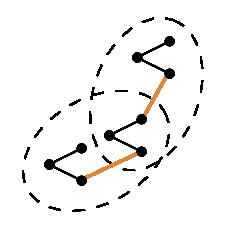
\includegraphics[height=0.5\textheight]{./assets/data_ecosystem_architecture.drawio.pdf}
                    \caption{Data Ecosystem}
                \end{figure}
            }
        \end{column}
    \end{columns}
\end{frame}


\begin{frame}{Data Spaces IV \footnotesize\cite{mollerIndustrialDataEcosystems2024}}
    \begin{itemize}
        \item flexible betriebliche Strukturen
        \item Zugang nur für bestimmte Akteure $\to$ \emph{Trusted Pool}
        \item sicheres, vertrauenswürdiges Data Sharing
        
        \pause
        \item Einbettung in Data Ecosystem
        \item \emph{Data Space Member} vs. \emph{Data Ecosystem Party}
        % DSM: direkt technisch in DS eingebunden
        % DEP: nur indirekter Zugriff über Data Space Connector (Schnittstelle zu DSM)
        
        \pause
        \item Governance"=Maßnahmen auf allen Abstraktionsebenen
        % Erfüllung rechtlicher Rahmenbedingungen
        % Ebene von DE, DS oder Use Case
    \end{itemize}
    
    % Data Spaces erfüllen am meisten Kriterien
    % Wie kann das funktionieren? --> Social Linked Data
\end{frame}

% !TeX root = ../presentation.tex

\section{Solid}

% TODO: Dreiecksbild auf meisten Folien klein in Ecke für Ref.

\begin{frame}{Solid \footnotesize\cite{mecklerWebLinkedData2023}}
    \begin{columns}
        \begin{column}{0.6\textwidth}
            \begin{itemize}
                % mögliche Implementierung des Data Space Konzeptes basiert auf Solid
                \item Data Space Konzept basierend auf\\
                    \emph{Solid} (ehem. Social Linked Data)
                    % TODO: Herkunft von Social Linked Data
                \item<2-> Ziel: offene, dezentralisierte Netzwerke für souveränen Datenaustausch
                \item<3-> Definition von Protokollen für Verwaltung und Austausch von Daten, Zugriffskontrolle und Identitätsmanagement
            \end{itemize}
        \end{column}
        
        \begin{column}{0.4\textwidth}
            \begin{figure}
                
\includegraphics[width=0.5\textwidth]{./assets/solid_logo.pdf}
                \caption{Solid-Logo~\cite{solidcommunitygroupSolidemblemsvg2019}}
            \end{figure}
        \end{column}
    \end{columns}
\end{frame}


\begin{frame}{Solid II \footnotesize\cite{mecklerWebLinkedData2023}}
    \vspace{1em}
    \begin{figure}
        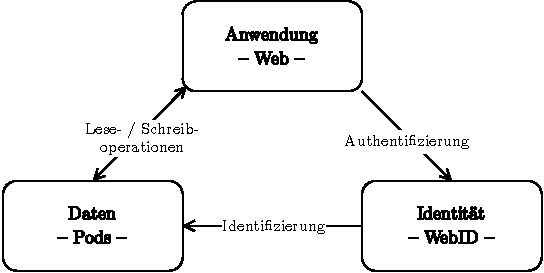
\includegraphics[height=5cm]{./assets/solid_triangle.drawio.pdf}
        \caption{Solid-Komponenten}
    \end{figure}
    % - Gliederung von Anwendungen in drei Teile
    %   - Anwendung als solches // Daten // Identität
    % - Identitätskomp.: verifiziert Identität eines Akteurs zur Auth. für Datenzugriff
    % - Daten und zugehörige Zugriffsregeln: dezentral in einen oder mehreren *Personal Online Data Stores* (Pods) gespeichert
    % - Anwendung verwendet ID, um korrekten Pod zu identifizieren und um sich für Datenzugriff zu auth.
    % - anschließend kann Anw. erforderliche Daten aus Pods lesen/schreiben
\end{frame}


\begin{frame}{Solid III \footnotesize\cite{mecklerWebLinkedData2023}}
    \begin{columns}
        \begin{column}{0.4\textwidth}
            \begin{itemize}
                \item Trennung und Standardisierung
                \item[$\Rightarrow$] Austauschbarkeit von Komponenten
                \item[$\Rightarrow$] Schritt"=für"=Schritt"=Einführung
                
                \item[$\Rightarrow$]<2-> geringe Einstiegsbarriere
                \item[$\Rightarrow$]<2-> hohe Zugänglichkeit
            \end{itemize}
        \end{column}
        
        \begin{column}{0.6\textwidth}
            \begin{figure}
                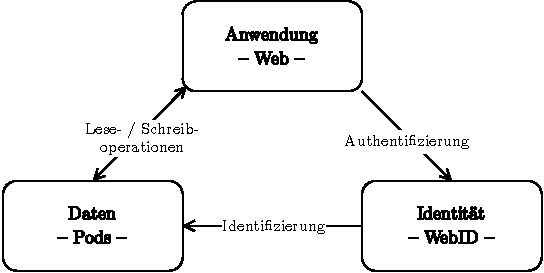
\includegraphics[width=\textwidth]{./assets/solid_triangle.drawio.pdf}
                % an Tafel malen
            \end{figure}
        \end{column}
    \end{columns}
\end{frame}


\subsection{Datenmanagement und Datenzugriff}

\begin{frame}{Datenstruktur}
    \begin{itemize}
        \item dezentrale Speicherung in \emph{Personal Online Data Stores} (Pods)~\cite{mecklerWebLinkedData2023,sambraSolidPlatformDecentralized2016}
        \item Standardisierung $\to$ Interoperabilität auf Daten"= statt Anwendungsebene
        % --> einfacher Wechsel von Anwendungen ohne aufwendige Datenmigration
        
        % \item Binärdaten\only<1|handout:0>{?} \only<2->{mit Metadaten}
        \item \only<1|handout:0>{Binärdaten?}
              \only<2>{Binärdaten mit Metadaten}
              \only<3-|handout:0>{\st{Binärdaten mit Metadaten}}
        
        \pause
        \pause
        \item lesbares Format \only<4->{$\to$ \emph{Resource Description Framework} (RDF) mit \emph{Vocabularies}~\cite{mecklerWebLinkedData2023,sambraSolidPlatformDecentralized2016}}
        % bspw. <Tim Berners-Lee> <is a> <person> (vgl. Bizer)
        % TODO: RDF-Erklärung höchstens kurz !!!
        
        \pause
        \pause
        \item Verknüpfung via \emph{Linked Data} $\to$ Struktur \& automatisierbare Semantik~\cite{bizerLinkedDataStory2009,mecklerWebLinkedData2023}

        \pause
        \item global eindeutige Identifikation via \emph{Uniform Resource Identifier} (URI)~\cite{sambraSolidPlatformDecentralized2016}
        \begin{itemize}
            \item \texttt{https://www.w3.org/People/Berners-Lee/card\#i}~\cite{bizerLinkedDataStory2009}
            % TODO: Unterschied URL / URI
        \end{itemize}
        
        \pause
        \item Zugriffskontrolle auf jeder Hierarchie-Ebene mittels \emph{Access Control List} (ACL)
        
        \pause
        \item Mapping anderer Strukturen zu RDF~\cite{mecklerWebLinkedData2023,sambraSolidPlatformDecentralized2016}
    \end{itemize}
\end{frame}


% \begin{frame}{Datenstruktur II \footnotesize\cite{mecklerWebLinkedData2023,sambraSolidPlatformDecentralized2016}}
%     \begin{columns}
%         \begin{column}{0.6\textwidth}
%             \begin{itemize}
%                 \item (nicht-) RDF"=Dateien in \emph{LDP"=Container}
%                 \item wiederum RDF"=Graph $\to$ Verschachtelung möglich
%                 \item Zugriffskontrolle auf jeder Ebene mittels \emph{Access Control List} (ACL)
%                 \begin{itemize}
%                     \item \texttt{resource.acl} oder \texttt{.acl}
%                 \end{itemize}

%                 \item<2> unterschiedliche Rechte pro Akteur / Container
%                 \item[$\Rightarrow$]<2> feingranularer Datenschutz und Zugriffskontrolle
%             \end{itemize}
%         \end{column}

%         \begin{column}{0.4\textwidth}
%             \vspace{1em}
%             \begin{figure}
%                 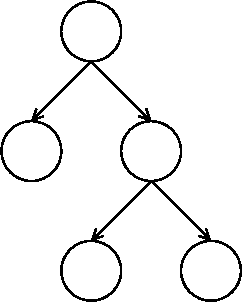
\includegraphics[height=4.5cm]{./assets/container_hierarchy.drawio.pdf}
%                 \caption{Hierarchie \cite[vgl.][]{sambraSolidPlatformDecentralized2016}}
%             \end{figure}
%         \end{column}
%     \end{columns}
% \end{frame}


\begin{frame}{Read- und Write-Protokoll \footnotesize\cite{mecklerWebLinkedData2023,sambraSolidPlatformDecentralized2016}}
    \begin{itemize}
        \item Anwendungen lesen und schreiben Daten direkt aus Pods
        \item Interoperabilität der Pods mit Anwendungen\\
            und wohldefiniertes, einfach implementierbares Protokoll
            % möglichst viel wiederverwenden, was bereits vorhanden ist
            % soll keine neue Komponenten sein --> aufbauend auf RESTful
        \item[$\Rightarrow$]<2-> RESTful"=Service, welche \emph{Linked Data Platform} (LDP) erfüllen
        \begin{itemize}
            % LDP: beschreibt Datenformat
            %   Einteilung in Ressourcen und Containern, Paging
            \item<2-> \texttt{HTTP GET}, \texttt{POST}, \texttt{PATCH}, \texttt{DELETE} etc.~\cite{sambraSolidPlatformDecentralized2016}
        \end{itemize}

        \item<3-> komplizierte Datenabfragen mittels SPARQL (optional)
    \end{itemize}
\end{frame}

% Fazit
% Datenmanagement betrachtet
% dezentrale Speicherung, Interoperabilität auf Daten- statt Anw.-Ebene
% Wie identifizieren wir Datenspeicher und Akteure für Datenzugriff? 

% \begin{frame}{Datenabfragen \footnotesize\cite{sambraSolidPlatformDecentralized2016}}
%     \begin{itemize}
%         \item nur einfache Abfragen mittels LDP"=Methoden möglich
%         \item komplizierte Datenabfragen mittels SPARQL (optional)
%         \item Delegation an Server $\Rightarrow$ Entwicklungsaufwand $\downarrow$

%         \pause
%         \item \emph{Local Queries}: innerhalb \emph{eines} Pods
%         \item \emph{Link Following Queries}: über mehrere Pods hinweg
%         \begin{itemize}
%             \item via Link"=Following
%             \item tatsächliche Verteilung muss nicht bekannt sein
%         \end{itemize}
%     \end{itemize}
% \end{frame}


\subsection{Identität und Authentifizierung}

\begin{frame}{Authentifizierung \footnotesize\cite{sambraSolidPlatformDecentralized2016}}
    \begin{itemize}
        \item Vertrauen, Datensouveränität und Datenschutz $\to$ Authentifizierung
        \item Dezentralisierung benötigt globalen \emph{Identity Space}
        
        \item<2-> passend zu RDF"=basierten Daten
        \item<2-> Ermittlung der Identität und Profildaten
        \item<2-> Ermittlung relevanter Links zum Pod und zu Anwendungsdaten
        
        \item[$\Rightarrow$]<3-> aktuell: \emph{WebID} (austauschbar)
        \item[$\Rightarrow$]<3-> globales Identitätsmanagement basierend auf System dezentralisierter \emph{Identity Provider}
    \end{itemize}
\end{frame}


\begin{frame}{Identität}
    \begin{columns}
        \begin{column}{0.55\textwidth}
            \begin{itemize}
                \item Akteure besitzen WebID"=URI~\cite{sambraSolidPlatformDecentralized2016}
                
                \item Referenz auf \emph{WebID Profile Document}~\cite{sambraSolidPlatformDecentralized2016,solidcommunitygroupSolidemblemsvg2019}
                
                \begin{itemize}
                    \item<2-> Referenz auf Pod und Anwendungsdaten~\cite{solidcommunitygroupSolidWebIDProfile2024}
                    \item<2-> Referenz auf weitere Profildaten~\cite{solidcommunitygroupSolidWebIDProfile2024}
                    % Webseite im RDF"=Format, global eindeutige URI~\cite{sambraSolidPlatformDecentralized2016}
                \end{itemize}
                
                \item<3-> Speicherung bei Identity Provider\\
                    (meist Pod Provider)~\cite{sambraSolidPlatformDecentralized2016}
                \item[$\Rightarrow$]<3-> Kontrolle über eigene Identität bei Nutzenden~\cite{sambraSolidPlatformDecentralized2016}
            \end{itemize}
        \end{column}

        \begin{column}{0.45\textwidth}
            \only<2->{
                \begin{figure}
                    \centering
                    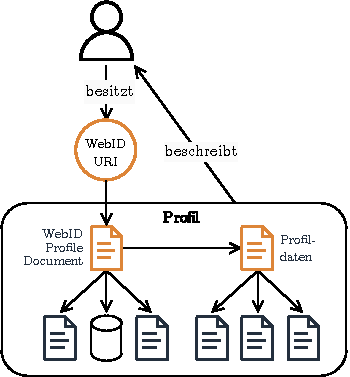
\includegraphics[height=5.5cm]{./assets/profile.drawio.pdf}
                    \caption{Solid Profil~\cite[vgl.][]{sambraSolidPlatformDecentralized2016,solidcommunitygroupSolidWebIDProfile2024}}
                \end{figure}
            }
        \end{column}
    \end{columns}
\end{frame}


\begin{frame}{Web of Trust \footnotesize\cite{sambraSolidPlatformDecentralized2016}}
    \begin{columns}
        \begin{column}{0.6\textwidth}
            \begin{itemize}
                \item Verknüpfung von Identitäten über mehrere Seiten\\
                $\Rightarrow$ \emph{Web of Trust}
                % hilfreich, da man nicht alle Akteure in einem DS / DE kennen kann
                
                \item[$\Rightarrow$]<2-> ad-hoc Auth.-Entscheidungen basierend auf Profileigenschaften
                % bspw. Beziehungen zu anderen Akteuren, Arbeitsstelle, Teil einer Gruppe etc. etc.
                % transitives Vertrauen
                
                \item[$\Rightarrow$]<3-> Wem kann ich vertrauen?\\ Kann ich den geteilten Daten vertrauen?
                
                \item[$\Rightarrow$]<4-> Adressierung eines Kern"=Hindernisses
            \end{itemize}
            % aber wenn ein Akteur kompromittiert, dann SCHLECHT
        \end{column}
        
        \begin{column}{0.4\textwidth}
            \vspace{1em}
            \begin{figure}
                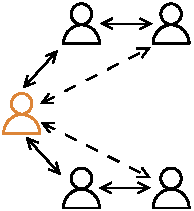
\includegraphics[height=4cm]{./assets/web_of_trust.drawio.pdf}
                \caption{Web of Trust}
            \end{figure}
        \end{column}
    \end{columns}
\end{frame}


\subsection{Erweiterung: Wertschöpfungsketten}

\begin{frame}{Erweiterung: Wertschöpfungsketten \footnotesize\cite{bothSolidBasedB2BData2025}}
    \begin{itemize}
        \item automatisierte Datenübertragung essenziell für Partner:in in Wertschöpfungsketten
        \item weitere Anforderungen
        \begin{itemize}
            \item garantierte, nachvollziehbare Einhaltung rechtlicher Rahmenbedingungen
            \item Constraints für Data Sharing
        \end{itemize}
    \end{itemize}

    \begin{figure}
        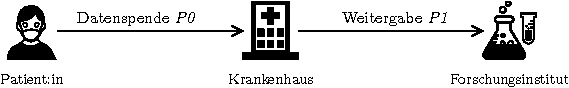
\includegraphics[width=\textwidth]{./assets/example_horizontal.drawio.pdf}
        \caption{Beispiel: Datenspende}
    \end{figure}
\end{frame}


\begin{frame}{Erweiterung: Wertschöpfungsketten II \footnotesize\cite{bothSolidBasedB2BData2025}}
    \addtocounter{figure}{-1}
    \begin{figure}
        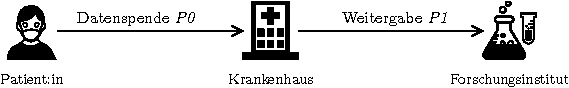
\includegraphics[width=\textwidth]{./assets/example_horizontal.drawio.pdf}
        \caption{Beispiel: Datenspende}
    \end{figure}
    
    \vspace{-1em}

    \begin{itemize}
        \item Einführung zusätzlicher Metadaten
        \begin{itemize}
            \item \emph{Data Processing Purpose} $P$ % Weitergabe muss sich trotzdem an ursprüngl. Zweck halte
            \item Verstecken der Datenquelle, Angabe über Weitergabe
        \end{itemize}

        \item<2-> weitere Validierung notwendig
        % weiterer Schritt in Richtung E2E-B2B-Wertschöpfungsketten
        % Möglichkeit und Notwendigkeit zur Erweiterung von Solid
    \end{itemize}

    % TODO: Stichpunkte zum Erzählen
\end{frame}

% !TeX root = ../handout.tex

\section{Verwandte Konzepte}

\begin{itemize}
    \item International Data Space, Gaia-X, Inter"=Organisational Information Systems
    \item \cite{mollerIndustrialDataEcosystems2024}
    \item \cite{sambraSolidPlatformDecentralized2016} \#Related Work
\end{itemize}

% !TeX root = ../presentation.tex

\section{Einschätzung und Zukunft}

\begin{frame}{Einschätzung}
    \begin{itemize}
        \item Zusammenführung vieler Ziele, um Vision näher an Realität zu bringen
        
        \pause
        \item Vertrauen?
        \pause
        \begin{itemize}
            \item Ansatz für Datensouveränität, Datensilos? gesetzliche Vorgaben?
        \end{itemize}
        % Ansatz zur Gewährleistung von Datensouveränität
        % unterschiedliche Datenspeicher je nach Kontext, Web of Trust
        % größerer Anreiz für Speicherung von Daten (<-- mehr Vertrauen und Kontrolle)
        % Web of Trust: ein kompromittierter Akteur reicht, um Schaden anzurichten
        % Startpunkt, aber wie verhindern, dass Data User die Daten zwischenspeichern?
        % Einhaltung gesetzlicher Vorgaben? --> o.g. Ansatz (Metadaten) benötigt weitere Forschung

        \pause
        \item Aktualität und Konsistenz von Daten?
        \pause
        \begin{itemize}
            \item Dezentralisierung und Datensouveränität, Anreiz $\uparrow$, Standardisierung
        \end{itemize}
        % mehr Vertrauen + Dezentralisierung + Datensouveränität 
        %     --> Daten bei Nutzenden
        %     --> größerer Anreiz zum Speichern von Daten
        % können diese einfach aktuell halten
        %     im Vgl. zu zentralisierten Ansatz, wo dieselben Daten verteilt bei vielen Unternehmen liegt
        % Standardisierung --> größere Verfügbarkeit von Daten

        \pause
        \item Effizienz und Geschwindigkeit?
        \pause
        \begin{itemize}
            \item Interoperabilität, automatisierbare Semantik, ggf. Mapping
        \end{itemize}
        % standardisierte Speicherung von Daten
        % Interoperabilität auf Daten- statt Anwendungsebene
        % automatisierbare Semantik durch RDF + Vocabularies
        % dadurch schnellere Datenintegration möglich, ggf. Mapping notwendig (teil- / automatisiert)

        \pause
        \item Zugänglichkeit unabhängig von Größe, Branche etc.?
        \pause
        \begin{itemize}
            \item Interoperabilität, Aufwand $\downarrow$, niedrigere Einstiegsbarriere

            \pause
            \item[$\Rightarrow$] Förderung von Kooperation und Innovation
        \end{itemize}
        % Interoperabilität auf Daten- statt Anw.-Ebene
        %     --> keine eigenen Daten mehr notwendig
        %     --> Zugänglichkeit von Daten
        % verminderter Aufwand durch Auslagerung von Std.-Fkt. + Wiederverwendbarkeit
        % niedrigere Einstiegsbarriere
        % Zugänglichkeit des Marktes
    \end{itemize}
\end{frame}


\begin{frame}{Zukunft}
    % TODO: Beispiel durchziehen
    % stellen uns vor: cooles neues Projekt
    % gehe zu neuen potenziellen Gesch.-Partnern und bringe meine Akten-Tasche voller Daten mit
    % ich kann alle meine Daten immer mit mir führen

    % dafür müssen sie digital sein

    \begin{itemize}
        \item Digitalisierung zum Profitieren von Vorteilen
        % digitales Bild nicht ausreichend, brauchen Daten mit automatisierbarer Semantik

        % interoperabel zur einfachen Zusammenführung
        \pause
        \item Dezentralisierung und Interoperabilität
        \begin{itemize}
            \item[$\to$] Fokus auf dezentrale Architekturen
        \end{itemize}

        % damit ermögliche ich ...
        \pause
        \item Ermöglichung von ad"=hoc Daten- und Anwendungsintegrationen
        \begin{itemize}
            \item[$\to$] Mapping statt aufwendige ETL"=Prozesse
                % Wiederverwendung, Schnittstellen
            
            % dyn. Interpr. durch Semantik aus RDF-Daten -->
            \item[$\to$] Abstraktion von Domänen-Daten, Metaprogrammierung
            % Branchen-agnostische Daten
            % Zukunft: Agenten interpretieren Daten nach meinen Kriterien, unabh. ob es User, Patient oder Benutzer heißt
        \end{itemize}

        % wird begünstigt durch
        \pause
        \item Datenstrukturen unabhängig von Anwendungen, Verfügbarkeit von Daten
        \begin{itemize}
            % aktuell: Wenn ich das mache, gehen Kunden weg?
            %          Einsperren von Kunden durch proprietäre Datenformate
            \item[$\to$] neue Art und Weise der Unterscheidung auf Markt
            \item[$\to$] Nutzerzentrierung, steigender Qualitätsanspruch
            % gutes Produkt zieht Kund. an, schlechtes stößt ab
            % begünstigt durch niedrigere Einstiegshürden in Markt
            % TODO: Blocker: Big Player werden dagegen wirken
        \end{itemize}

        \pause
        \item[$\Rightarrow$] Daten-orientiertes Vorgehen statt Prozess-Orientierung
        % Daten als Antreiber statt Prozesse
    \end{itemize}
\end{frame}

% !TeX root = ../handout.tex

\section{Fazit}

In diesem Handout wurden Data Spaces vorgestellt, welche dezentrale, multilaterale Informationssysteme anstreben, um ein vertrauenswürdiges Data Sharing unter Garantie von Datensouveränität zu ermöglichen.
Eine mögliche Umsetzung basiert auf dem offenen Standard Solid, welcher die Verwaltung und den Austausch von Daten und Identitäten definiert.
Daten werden dezentral in Pods gespeichert, wobei die volle Kontrolle über den Zugang bei Nutzenden liegt.
Durch Standardisierung und Interoperabilität können Datenspeicher unabhängig von Anwendungen gewechselt werden.
Authentifizierungsentscheidungen können ad-hoc über ein Web of Trust getroffen werden.
Somit soll ein vertrauenswürdiges Teilen von aktuellen und konsistenten Daten als Basis für effiziente Integrationen ermöglicht werden.
Zukünftig könnte dies in Richtung vollständige Digitalisierung, Metaprogrammierung mit agnostischen Daten sowie Nutzerzentrierung von Anwendungen führen.


\printbibliography[heading=bibintoc, title=Quellenverzeichnis]

% \appendix

\end{document}
\endinput
